\section{\$P-recognizer}

In this algorithm, we consider each gesture as a set of points: $\set{p_i = (x_i, y_i) : i = 1,...,N}$. In our case, because of the resampling made in the preprocessing step, each gesture is represented by a set of $N = 32$ points. It is worth noticing that gesture are seen as a cloud of points so that there does not need to have order in the set (i.g. $p_1$ does not have to be the starting point nor $p_{i}$ has to follow $p_{i-1}$) even though it's the case for us. 

Let $C$ and $T$ be clouds of points. The first one correspond to a gesture candidate whereas the second one is a template in the training set. The aim of this algorithm is to match $C$ to $T$ by the use of a nearest neighbor classifier (KNN) in the same idea as the precedent section. Here we obviously do not use a dtw algorithm to compute the distance but the sum of euclidean distances for all pairs of points $(C_i, T_j)$ where $C_i \in C$ is matched to $T_j \in T$ through some function $f: \R^2 \rightarrow \R^2, \quad C_i \rightarrow f(T_j)$,
\begin{equation}
	d(C, T) = \sum_{i=1}^{N} ||C_i - T_j||_2
\end{equation}

However this algorithm requires to search for the minimum matching distance between $C$ and $T$ from $n!$ possible alignments. The library we used to run this algorithm uses a special heuristic called Greedy-5 (\cite{Vatavu_Anthony_Wobbrock_2012}). The idea is that for each point $C_i \in C$, we find the closest point in $T$ that has not been matched yet. Once it is matched with $C_i$, we continue with $C_{i+1}$ and so on until all the points of $C$ are matched with a point of $T$. The closeness is computed through a weighted euclidean distance,
\begin{equation}
	d(C, T) = \sum_{i=1}^{N} w_i ||C_i - T_j||_2
\end{equation}
where $w_i$ indicate the confidence in each pair $(C_i, T_j)$.

Basically, the first match has a weight of $1$ since $C_i$ has all the points of $T$ to choose for the closest match. As long as the possibility of matching reduces, the confidence also. The formula for the weights translates a linearly decreasing weighting,
\begin{equation}
	w_i = 1 - \frac{i - 1}{N}
\end{equation}

This heuristic allows us to have a time complexity of $\mathcal{O}(n^{2 + \epsilon})$ which is comparable to the standard dtw algorithm without any optimization.

\subsection{Results}

\subsubsection{User-independent cross-validation}

For the first domain, we get a mean accuracy of $0.925$ along with a standard deviation of $0.029$ for the user-independent cross-validation. This is way better than with the dtw algorithm even though we had resample the datas with half the number of data points than for the precedent algorithm. Notice that we do not have anymore the problem of a split containing a lot of missclassifications as we had in dtw.

\begin{figure}[H]
	\centering
	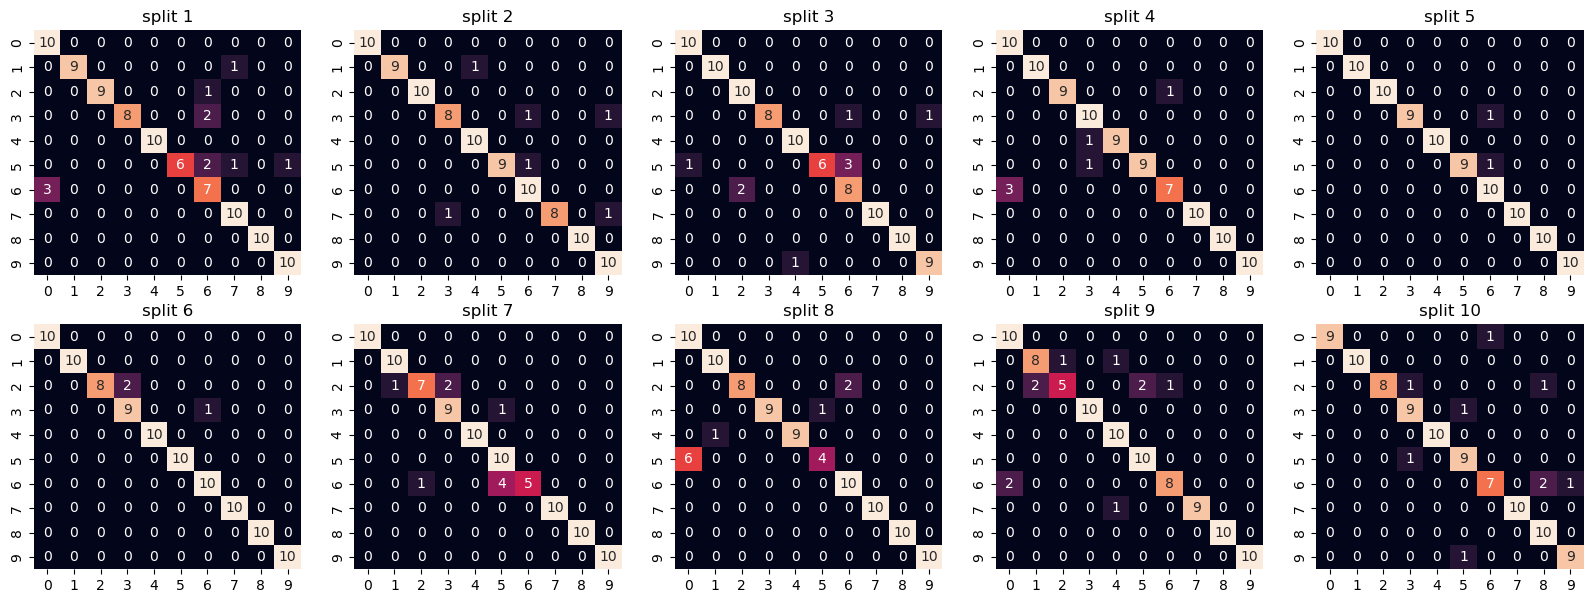
\includegraphics{figures/pcr/domain01/cm_pcr_d1_uindep.png}
	\caption{Confusion matrices of the different splits for the domain 1 using \$P-Recognizer algorithm (user independent cross-validation)}
	\label{fig:cm-pcr-d1-uindep}
\end{figure}

For the third domain, we get a mean accuracy of $0.971$ along with a standard deviation of $0.021$. This is slightly better than for the first domain despite this one has more complex shape to recognize.

\begin{figure}[H]
	\centering
	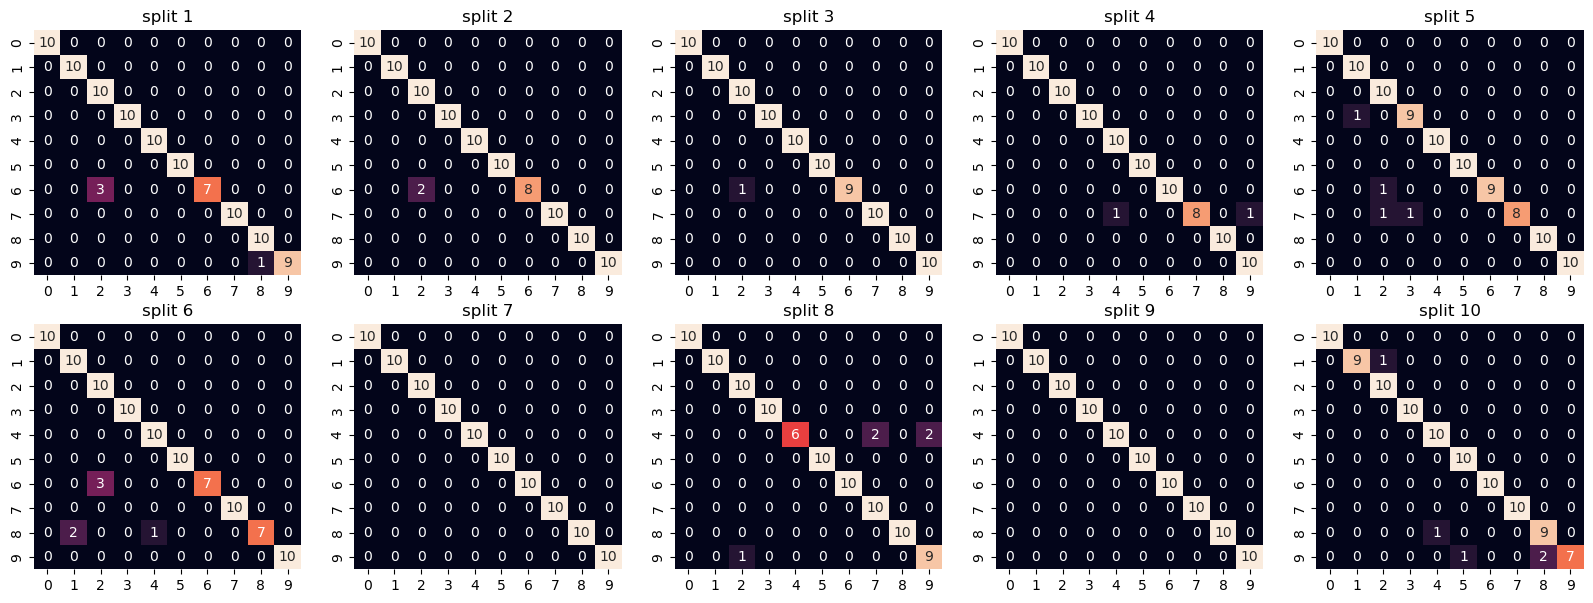
\includegraphics{figures/pcr/domain03/cm_pcr_d3_uindep.png}
	\caption{Confusion matrices of the different splits for the domain 3 using \$P-Recognizer algorithm (user independent cross-validation)}
	\label{fig:cm-pcr-d3-uindep}
\end{figure}

\subsubsection{User-dependent cross-validation}

For the first domain, we get a mean accuracy of $0.967$ with a standard deviation of $0.02$ and for the third domain, we get a mean accuracy of $0.99$ along with a standard deviation of $0.01$. The results are somewhat comparable to those of dtw for the user-dependent setting.

\begin{figure}[H]
	\centering
	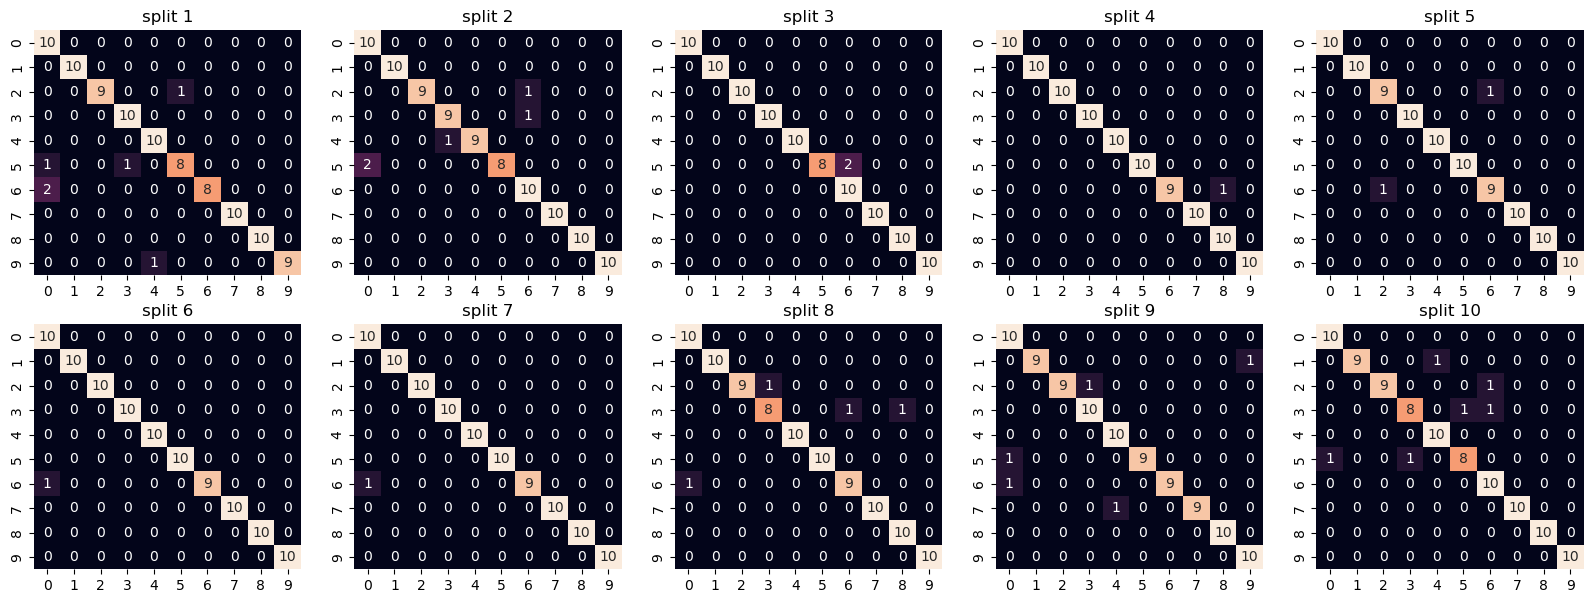
\includegraphics{figures/pcr/domain01/cm_pcr_d1_udep.png}
	\caption{Confusion matrices of the different splits for the domain 1 using \$P-Recognizer algorithm (user dependent cross-validation)}
	\label{fig:cm-pcr-d1-udep}
\end{figure}

\begin{figure}[H]
	\centering
	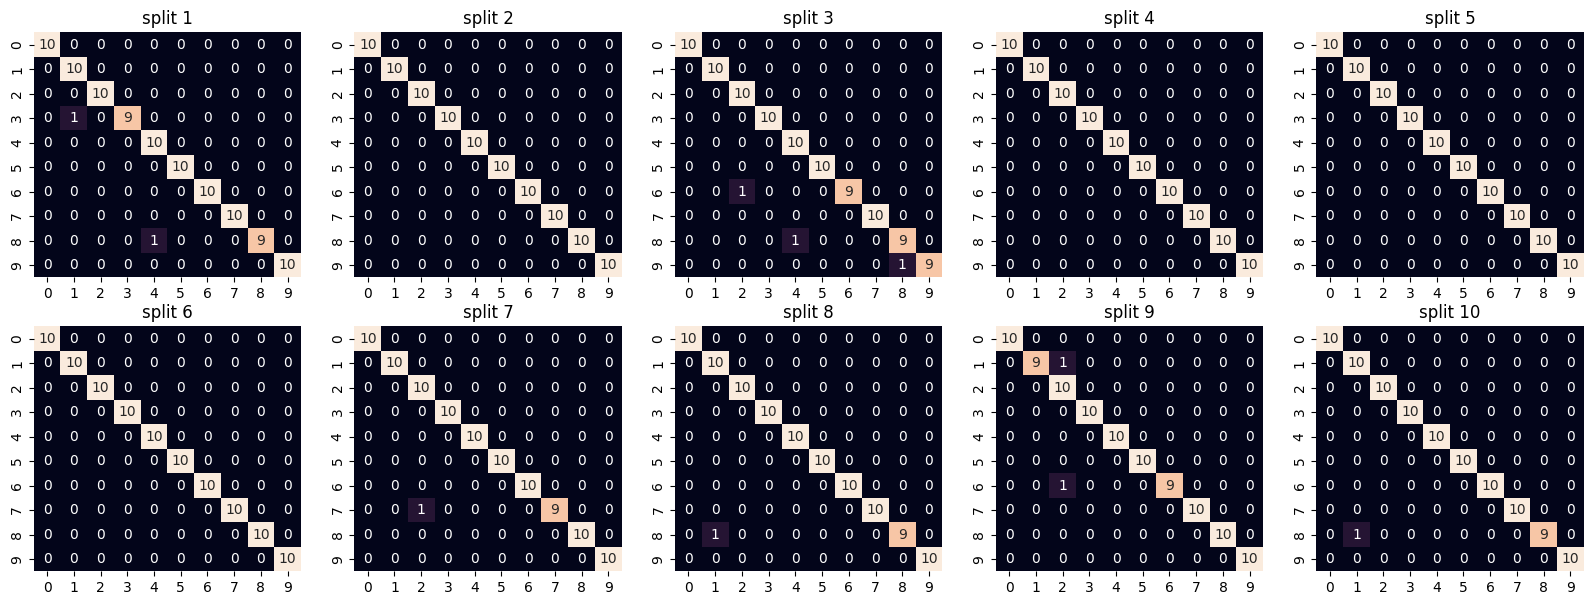
\includegraphics{figures/pcr/domain03/cm_pcr_d3_udep.png}
	\caption{Confusion matrices of the different splits for the domain 3 using \$P-Recognizer algorithm (user dependent cross-validation)}
	\label{fig:cm-pcr-d3-udep}
\end{figure}